We next compare group lasso, GrOWL-I and GrOWL-II by analyzing synthetic data generated
from a deep neural network model trained to generate distributed representations of a
word's sound (phonology) and meaning (semantics) from its spelling (orthography;
Figure~\ref{fig.network} top left). The network structure is motivated by the influential
``triangle'' model of the human reading system \citep{PlautETAL96}. Specifically,
phonological outputs receive contributions from two separate pathways: a {\em direct} route
mediated by a single hidden layer, and an ``indirect'' route composed of three hidden
layers, which must first compute mappings from orthography to semantics, then project
onward to contribute to the phonological outputs. This architecture is interesting because
different kinds of similarity structure emerge through learning in different network
components. The central idea is that orthographic and phonological similarities are highly
systematic: items that are similar in spelling are likely (though not guaranteed) to be
similar in pronunciation. These regularities are easily learned within the direct pathway
mapping from orthography to phonology, allowing the system to generate appropriate
pronunciations for previously unseen word-forms. In contrast, orthographic and semantic
similarity structures are unsystematic: similarity of word spelling does not necessarily
predict similarity of meaning and vice versa. In learning to map from orthography to
semantics and on to phonology, the indirect path thus comes to encode quite different
similarity relations amongst the words than does the direct
path \citep{PlautETAL96,HarmSeidenberg04}.

To capture these properties we generated model ``orthographic'' representations as patterns
sampled from 6 overlapping clusters of binary input features, roughly corresponding to
different orthographic neighborhoods. For every word a ``phonological'' pattern was
generated by flipping each orthographic feature with probability 0.1. Thus phonological
patterns were distorted variants of orthographic patterns, creating high systematicity
between these. We also created a ``semantic'' pattern for each word from a set of binary
features also organized into clusters. Across items, these vectors expressed a hierarchical
similarity structure with two broad superordinate clusters each composed of three tighter
clusters. Importantly, the similarity structure expressed by the semantic vectors was
independent of the structure expressed in the orthographic/phonological patterns. The left
bottom panel in Figure~\ref{fig.network} shows the cosine distances encoded amongst the 30
``words'' in each layer of one trained model. Layers in the direct path each encode roughly
the same distances amongst items, while the semantic layer encodes a quite different set of
distances that is weakly reflected in two of the three hidden layers in the indirect path.
Thus the different components of this simple word-reading network contribute differentially
to the encoding of semantic versus ortho-phonological similarity structure.

We trained 5 models with different initial weights, corresponding to 5 model subjects, and
presented each with 30 orthographic inputs. Each input generated a vector of activations
over the 100 model units. To ensure high redundancy amongst units this vector was
concatenated 5 times and perturbed with independent noise, yielding 500 measurements per
model subjects. These were treated as analogs of the estimated BOLD response at each of 500
model voxels in a brain imaging study. We then applied group lasso and GrOWL to find the
voxel subsets that encode either the semantic or phonological distances (derived from the
target values for the semantic and phonological output layers of the network). We fit
models by searching a grid of parameters ($\lambda$, $\lambda_1$), including $\lambda_1=0$
as the special case of GrOWL that is group lasso. For each grid point we counted a voxel as
``selected'' if it received a non-zero weight, and assessed how accurately the model
selected  the voxels encoding phonological structure (all those along the direct pathway)
or semantic structure (the semantic layer hidden layers 2 and 3 in the indirect path) by
computing hit rates and false alarm rates. All three models showed low and equivalent
cross-validation error; however GrOWL-II achieved this error rate while selecting
considerably more voxels. The ROC plots in Figure~\ref{fig.roc} further show that GrOWL-II
did not select additional voxels at random: it outperformed group LASSO considerably in
discriminating signal-carrying from non-signal carrying voxels. The right panel of
Figure~\ref{fig.network} shows the frequency with which each model unit is selected for the
best-performing solution of each method and structure type. The strong sparsity enforced by
group lasso is clearly apparent: target units are selected less consistently than with
GrOWL, which consistently discovers more of the signal.

Finally, we considered the ability of GrOWL to reveal the network structure encoding each
kind of similarity, treating the weights in the matrix $\bW$ as direct estimates of the
joint participation of pairs of units in expressing the target similarity. The rightmost
plots of Figure~\ref{fig.network} show the estimated connectivity, thresholded to show the
25\% of the non-zero weights with the largest magnitudes. The detected edges clearly
express the network representational substructure: units in the direct pathway are shown as
highly interconnected with one another and weakly or disconnected from those in the
indirect pathway, and vice versa. Thus the search for different kinds of similarity reveals
different functional subnetworks in the model.

\begin{figure*}[!t]
\centering
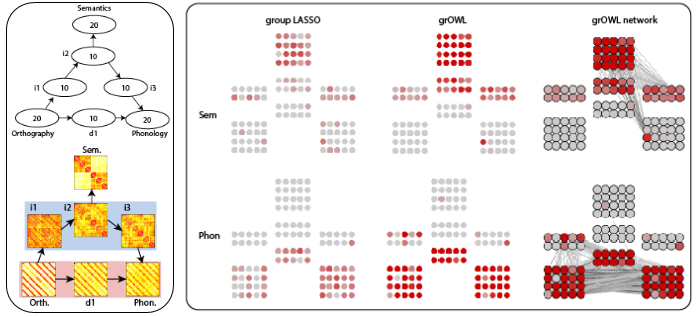
\includegraphics[width=0.99\textwidth]{figures/Network_results1.png}
\caption{Left panel: Network architecture (top) and the similarity structure expressed in
  each layer (bottom). Red background shows the direct pathway and blue the indirect
  pathway from orthography to phonology. Layers in the two pathways encode different
  similarity structures. The target similarity matrices for the analysis express either the
  semantic structure (top layer) or the phonological structure (bottom right layer). Arrows
  indicate feed-forward connectivity. Right panel: Units selected by group LASSO (right)
  and GrOWL (middle) when decoding semantic (top) or phonological (bottom) structure.
  Colors show the proportion of times across subjects and unit concatenations that the unit
  received a non-zero weight, with red indicating 1 and gray 0. The rightmost plots show
  the largest weights in the associated matrix W for each GrOWL model, which pick out two
  subnetworks in the model.}
\label{fig.network}
\end{figure*}

\begin{figure*}[!h]
\centering
\subfloat[]{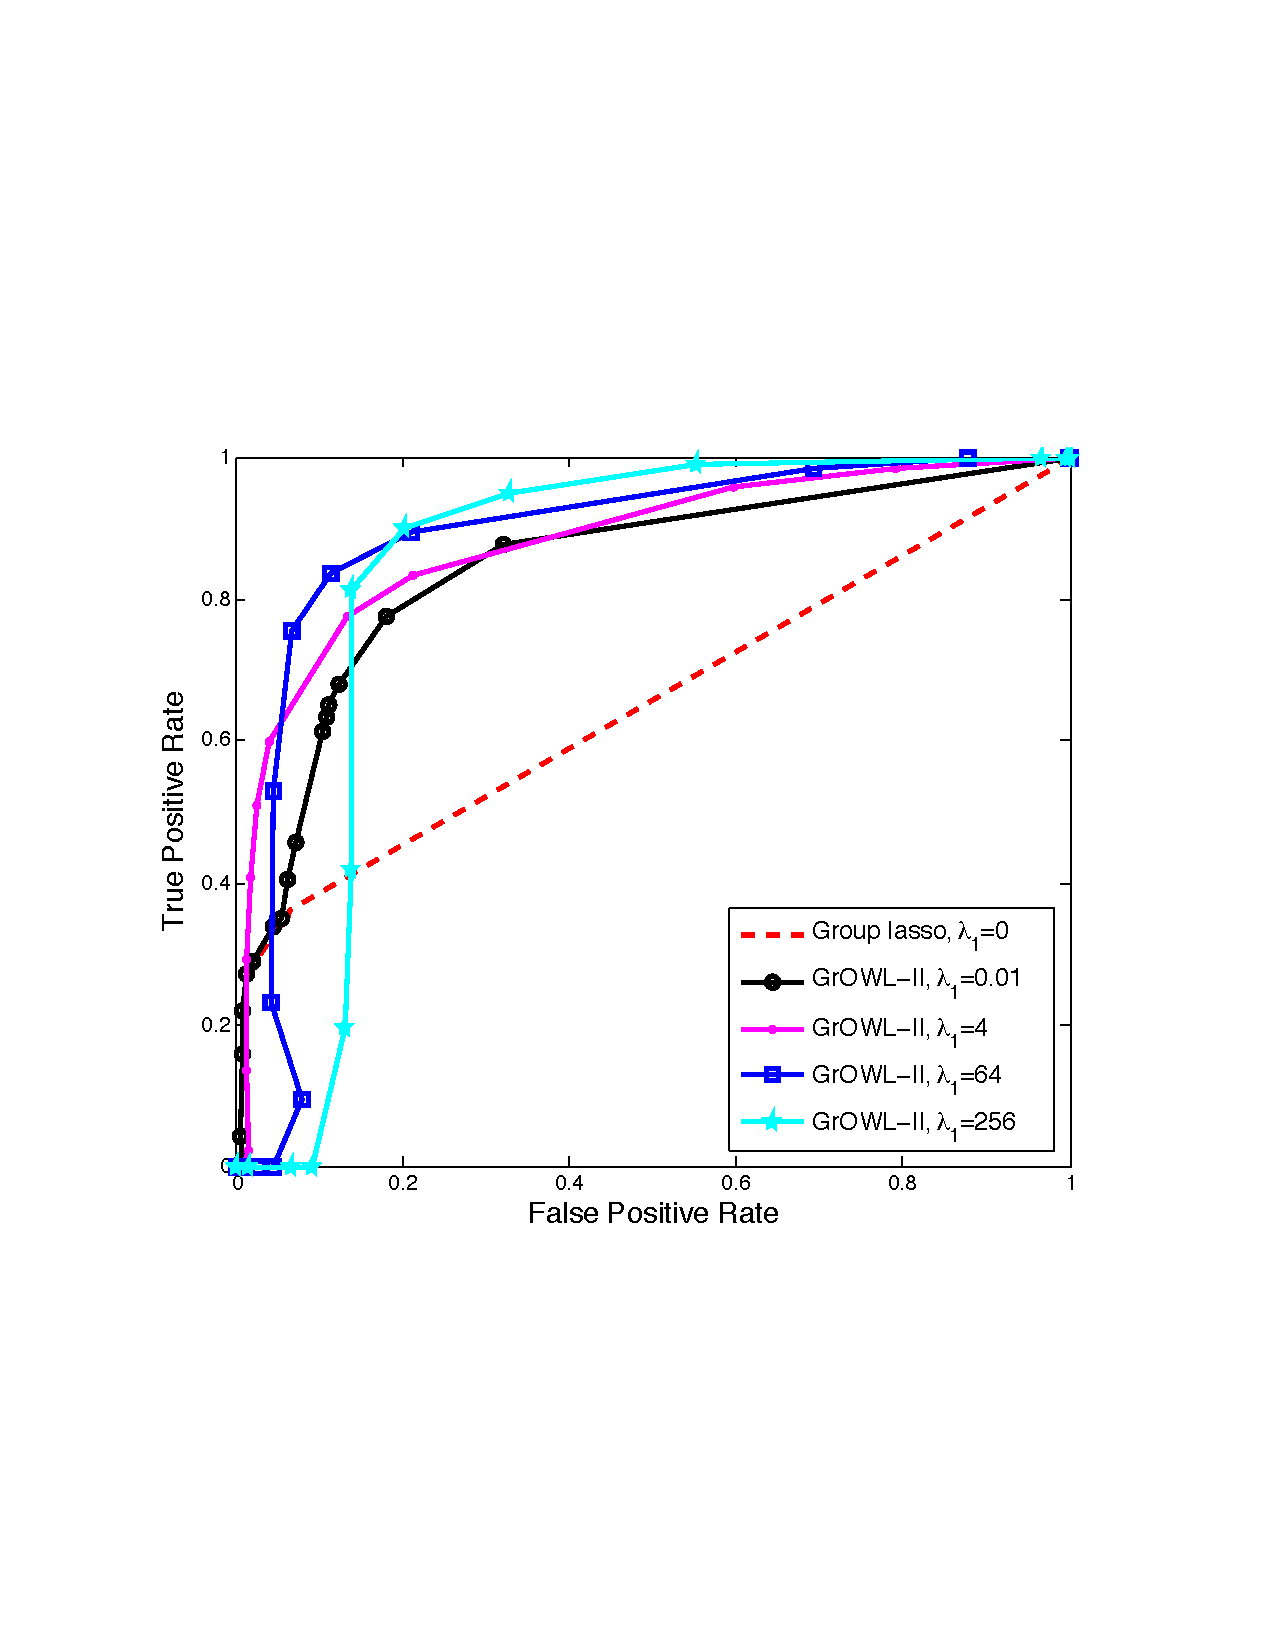
\includegraphics[width=0.4\textwidth]{figures/ROC_sem.pdf}
\label{fig_first_case_roc}}
\hfill
\subfloat[]{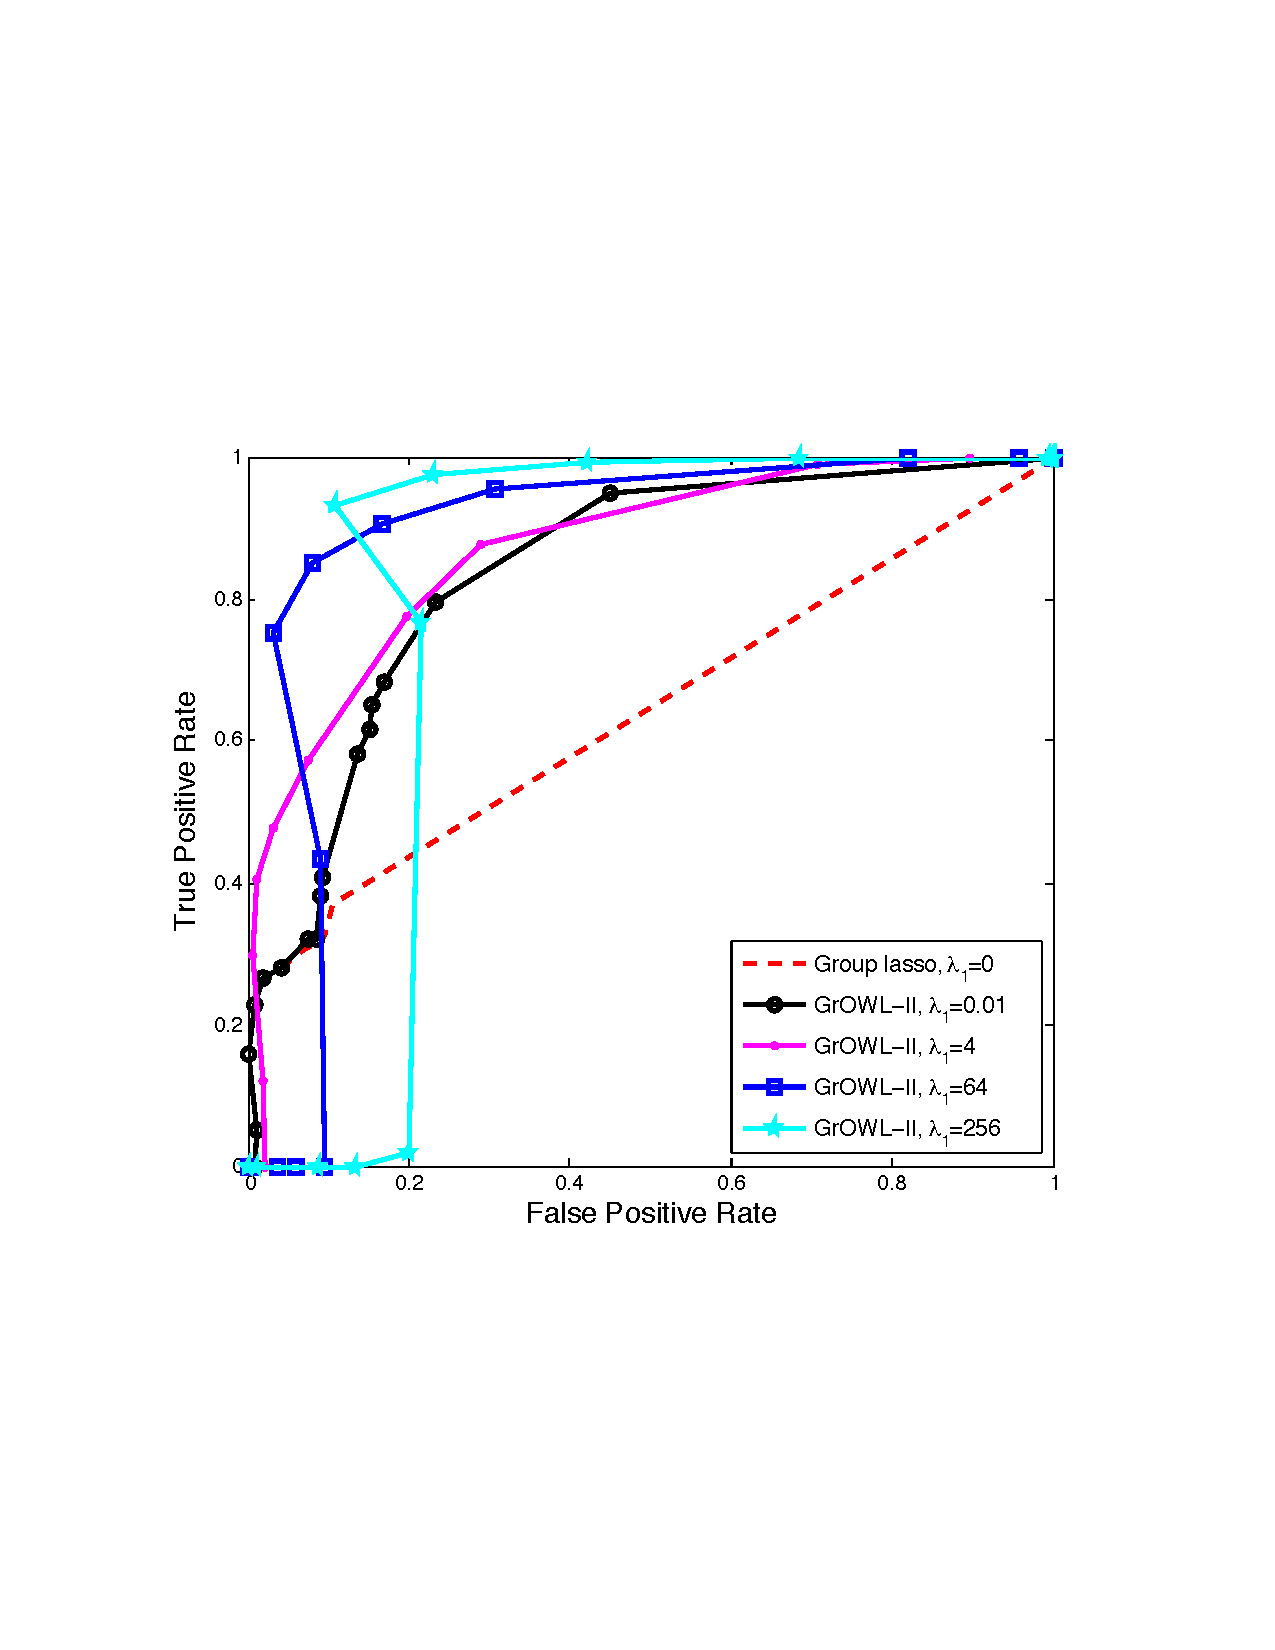
\includegraphics[width=0.39\textwidth]{figures/ROC_phon.pdf}
\label{fig_second_case_roc}}
\caption{ROC curves generated by sweeping through $\lambda$ values (for $\lambda = 0$, all
  units are selected and as $\lambda$ is increased fewer units are given non-zero weight).
  Each curve represents a fixed value of $\lambda_1$, where the curve $\lambda_1 = 0$
  corresponds to group lasso. ROC curves are averaged across participants for each method,
  considering both similarity structures, Semantics (left panel) and Phonology (right
  panel).}
\label{fig.roc}
\end{figure*}
